% Miktex Beamer template
% Author: Carl Schneider
% University TUDelft
% www.dutiosc.twi.tudelft.nl/~carl/
% or: http://www.ewi.tudelft.nl/live/pagina.jsp?id=3b29bfdd-1cb1-4e15-b03c-a5dab56837e2&
% April 2010

\documentclass{beamer}

% Necessary definitions:
\setbeamersize{sidebar width left=0.5cm}
%\usepackage[english]{babel}
\usepackage{tikz}
\usepackage{float}
\usepackage{hyperref}
\usepackage{tabularx}
\usepackage{tikz}
\usepackage{todonotes}
\usepackage{caption}
\usepackage[utf8]{inputenc}
\newcommand{\field}[1]{\mathbb{#1}}
\newcommand{\Zset}{\field{Z}}
\mode<presentation>
{\usetheme{Boadilla} % This theme will be adjusted into the TUDelft lay-out
 \setbeamercovered{transparent}}
\definecolor{tudblue}{rgb}{.004,.50,.78} % definition TUDelft blue color
\setbeamercolor{structure}{fg=tudblue}
\setbeamercolor{palette primary}{fg=white,bg=tudblue!85}       % Right field
\setbeamercolor{palette secondary}{fg=white,bg=tudblue!85}     % Middle field
\setbeamercolor{palette tertiary}{fg=tudblue!85,bg=tudblue!85} % Left field
\setbeamersize{text margin left=1cm}
\setbeamersize{text margin right=1cm}

%---------------------------------------------------------------------------------
%  Take attention for the parts you may change. See the comment lines with: %>>>
%---------------------------------------------------------------------------------

%>>> You may change the text in this part {Between brackets}:
%>>> This is for the Title page:
\newcommand*\titel{Robotic Swarms}
\newcommand*\subkop{Distributed Coordination Without Location}
\newcommand*\naam{S.J.A. Bekhoven, S.P. Metman, M.J. Rogalla}
\newcommand*\afdeling{EEMCS}
%>>> This is for the frame-title on the "Table of Contents" page:
\newcommand*\titelTOC{Outline}
%>>> This is for the frame-title on the "Table of Contents" page when the next subsection will start:
\newcommand*\subsectie{Next Subsection}


%%% Not change this part below %%%
%%% Title Page (belongs to the theme)%%%
% Necessary part for the theme:
\title{\titel} % This title also appears in the TUDelft bar on the next pages
\author[]{\naam}
\institute[]{\subkop \\ TU Delft}
\date[]{\today}
\AtBeginSubsection[]
{\begin{frame}<beamer>\frametitle{\textbf{\LARGE{\textrm{\subsectie}}}}
    \tableofcontents[currentsection,currentsubsection]  % Generation of the Table of Contents
\end{frame}}
\tikzset{textlabel/.style={color=white}}
\beamertemplatetransparentcovereddynamicmedium

%==============================================================
%%% Not change this part below, except maybe the folder where you placed the "TUDelft bies"
\begin{document}
% Adjusting boadilla theme lay-out to TUDelft lay-out:
\setbeamertemplate{sidebar left}  % blue square left above
{\vfill
\rlap{%\hskip0.1cm

\includegraphics[scale=0.33]{TUDelft/beamer-tudelft-bies.jpg} }
\vskip-5pt}

%--------------------------------------------------------------

% Section 0
% Subsection 0
% Page 1
% Title page
%%% This is the first frame of the presentation.
%%% Please do not change it except maybe the comment signs in case of a background photo
%%% and the place and name of the photo (
\begin{frame}
    \begin{tikzpicture} [remember picture, overlay]
        \node [shift={(0.5 cm,-5.35cm)}]  at (current page.north west)
        {
        \begin{tikzpicture}[remember picture, overlay]
            %%% These 2 coming lines you may uncomment if you want to have a photo on the background(2198x1480pixels) of the title page
            \node [shift={(-0.14cm,5.56cm)},right] at (current page.south west) % background photo
            {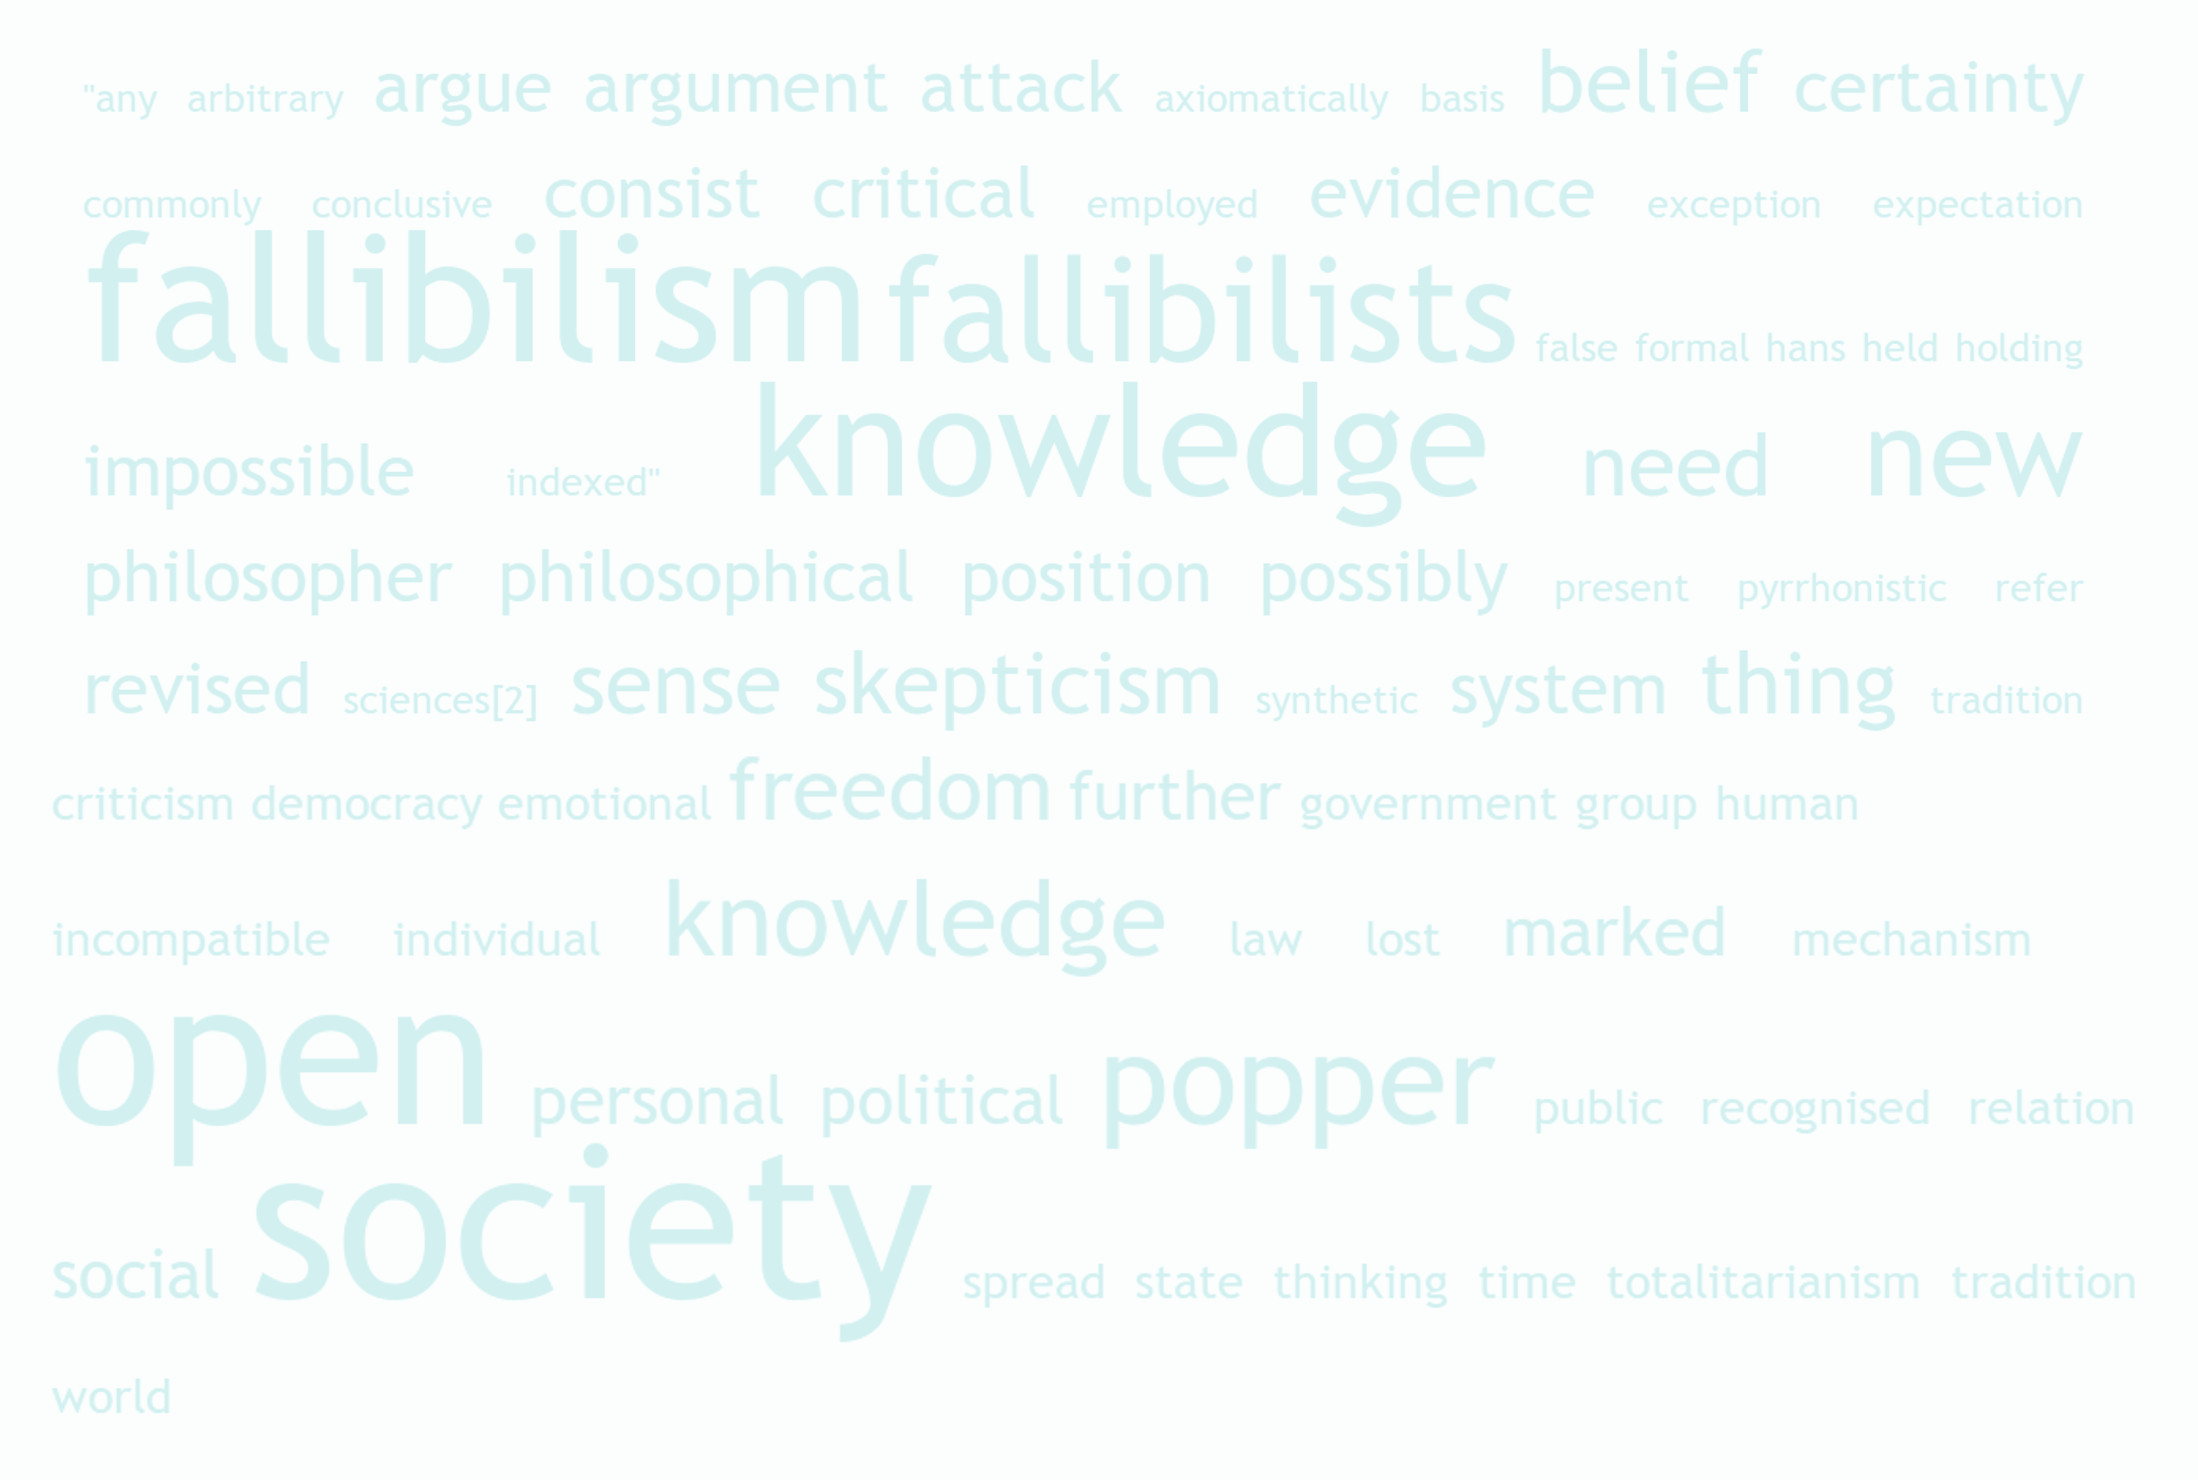
\includegraphics[height=8.65cm]{TUDelft/background-titlepage.jpg}};            % background photo
            \fill [cyan!95!black!70!blue] (0,2.9) -- (0,5.35) -- (-.5,5.35) -- (-.5,2.9) -- cycle ;%squareNorthWest
            \draw [fill=black] (0,0) -- (11,0) -- (11,2.9) -- (0,2.9) -- cycle ;
            \fill [fill=cyan!65!blue!80] (7,-3.9) -- (12.4,-3.9) -- (12.4,-3.65) -- (7,-3.65) -- cycle;
            \node [shift={(0.8cm,-2.9cm)},textlabel,right]  at (current page.north west) {\textbf{\LARGE{\textrm{\titel}}}};
            \node [shift={(0.8cm,-3.5cm)},textlabel,cyan!95!black!70!blue,right]  at (current page.north west)
            {\textbf{\large{\textrm{\subkop}}}};
            \node [shift={(0.8cm,-4.6cm)},textlabel,right]  at (current page.north west)
            {\normalsize{\naam, \afdeling}};
            \node [shift={(0.8cm,-5cm)},textlabel,right]  at (current page.north west)
            {\normalsize{\today}};
        \end{tikzpicture}};
    \end{tikzpicture}
\end{frame}

%--------------------------------------------
%%% Table of contents (TOC)
% The TOC will generated after building your section(s) and subsections
\begin{frame}<beamer>\frametitle{\textbf{\LARGE{\textrm{\titelTOC}}}}
    \begin{tikzpicture}[remember picture, overlay]
        \node [shift={(0.5 cm,-5.35cm)}]  at (current page.north west)
        {
        \begin{tikzpicture}[remember picture, overlay]
            \fill [fill=cyan!65!blue!80] (7,-3.9) -- (12.4,-3.9) -- (12.4,-3.65) -- (7,-3.65) -- cycle;
        \end{tikzpicture}};
    \end{tikzpicture}
    \tableofcontents
\end{frame}
%--------------------------------------------

\section{Introduction}
\begin{frame}\frametitle{\textbf{\LARGE{\textrm{Introduction}}}}
  \begin{itemize}
    \item What are Robotic Swarms?
    \item Why did we write this paper?
    \item How did we achieve this?
  \end{itemize}
\end{frame}

\section{Terminology}
\subsection{Swarm Definition}
\begin{frame}\frametitle{\textbf{\LARGE{\textrm{Swarm Definition}}}}
  \begin{itemize}
    \item Scalable Network of Robots
    \item More than 2 Robots
    \item Distributed Intelligence
  \end{itemize}
\end{frame}
\subsection{Location \& Range}
\begin{frame}\frametitle{\textbf{\LARGE{\textrm{Location \& Range}}}}
\begin{description}
  \item[Location-free]  \hfill \\ Robots have no knowledge of their absolute location but may keep track of their relative location.
  \item[Location-based]  \hfill \\Robots have perfect knowledge of their absolute location.
  \item[Range-free]  \hfill \\Robots do not communicate or communicate via some kind of central base.
  \item[Range-based]  \hfill \\Robots communicate within predetermined range.
\end{description}
\end{frame}
\subsection{Performance\& Scalability}
\begin{frame}\frametitle{\textbf{\LARGE{\textrm{Performance\& Scalability}}}}
\begin{description}
  \item[Performance] \hfill \\ The general efficiency, which is defined differently per problem.
  \item[Scalability] \hfill \\ The ability of maintaining performance when the population in the robot swarm is increased.
\end{description}
\end{frame}
\subsection{Problem Composition Overview}
\begin{frame}\frametitle{\textbf{\LARGE{\textrm{Main Problems vs. Composite Problem}}}}
%\begin{description}
  %\item[Composite Problem] \hfill \\ A composite problem is a problem composed of multiple main problems.
  %\item[Main Problem] \hfill \\ A main problem have overlap as well, but without significant impact.
%\end{description}
\begin{figure}
  \centering
  \begin{tikzpicture}[width=0.5\textwidth,->,>=stealth,shorten >=2pt,auto,node distance=3.5cm,
    thick,main node/.style={fill=white,draw,font=\sffamily}]
    \node at (7.7,0.75) {main problems};
    \node at (7,-3.45) {composite problems};
    \draw[fill=white,dashed] (-1.2,-2) rectangle (8.8,0.5);
    \draw[fill=white,dashed] (8.8,-3.2) rectangle (5.2,-2.3);
    \node[main node] (1) {Exploration};
    \node[main node] (2) [below= 0.9cm of 1] {Dispersion};
    \node[main node] (3) [right of=1] {Formation};
    \node[main node] (4) [right of=3] {Source Localization};
    \node[main node] (5) [below= 2.2cm of 4] {Collective Transport};

    \path[every node/.style={font=\sffamily\small}]
      (1) edge [right] node[left] {} (2)
      (4) edge [right] node[left] {} (3)
      (5) edge [right] node[left] {} (4)
      (5) edge [right] node[left] {} (3)
      (1) edge [right] node[left] {} (3);
  \end{tikzpicture}
  \caption{Problem Composition Overview} \label{fig:ProblemsOverview}
\end{figure}
\end{frame}
\begin{frame}\frametitle{\textbf{\LARGE{\textrm{Formation}}}}
\end{frame}

\section{Problems}
\subsection{Main Problems}
\begin{frame}\frametitle{\textbf{\LARGE{\textrm{Formation}}}}
\end{frame}
\begin{frame}\frametitle{\textbf{\LARGE{\textrm{Dispersion}}}}
\end{frame}
\begin{frame}\frametitle{\textbf{\LARGE{\textrm{Exploration}}}}
\end{frame}
\begin{frame}\frametitle{\textbf{\LARGE{\textrm{Source-localization}}}}
\end{frame}
\subsection{Composite Problems}
\begin{frame}\frametitle{\textbf{\LARGE{\textrm{Collective-transport}}}}
\end{frame}

\section{Discussion}
\begin{frame}\frametitle{\textbf{\LARGE{\textrm{Discussion}}}}
\end{frame}

\end{document} 
